\section{Control Configuration}

\subsection{Differential Drive}

Using two motors will consume less power than using four motors and the cost also will be the lower-cost. But it cannot completely complete some of the more complicated moves, such as some seas have more reefs and avoid the boat hitting the rocks, so it needs precise movement.

\[LeftMotor = Y + X\]
\[RightMotor = Y-X\]
\begin{figure}[h]
	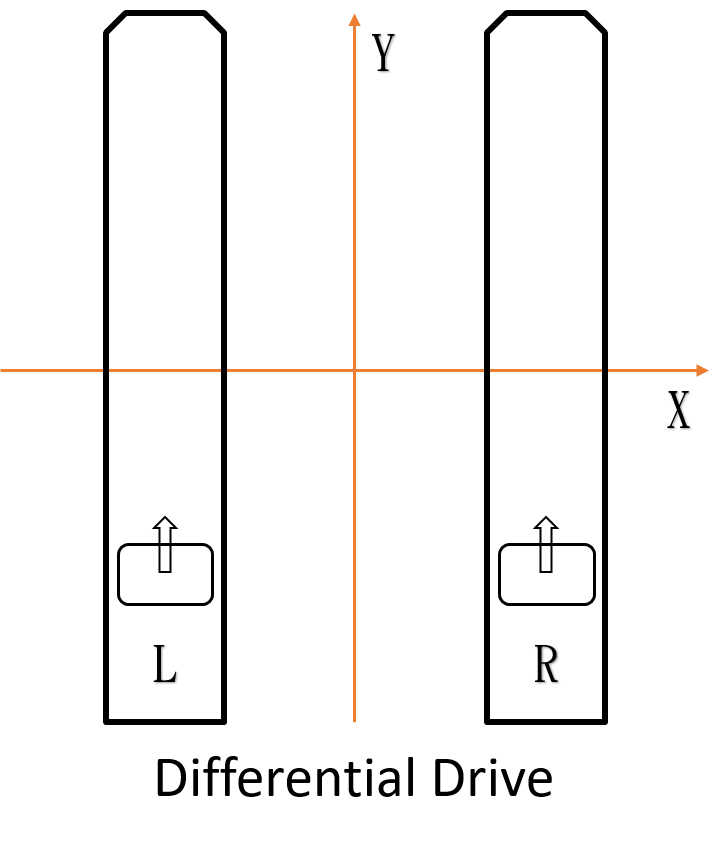
\includegraphics[width=0.5\columnwidth]{images/differential_drive.png}
	\centering
	\caption{differential drive motor config}
	\label{figure:differential_drive}
\end{figure}

\subsection{Omnidirectional Drive}

We choose to use four motors is because it can move omnidirectional, but it will consume more power and the motor is expensive will increase the cost of the Duckieboat. But it can move with precision, can be used in more complex environments.

\paragraph{Forward Kinematics}
\[Front Left Motor = Y + X + A \]
\[Front Right Motor = Y - X - A \]
\[Rear Left Motor = Y - X + A \]
\[Rear Right Motor = Y + X - A\]

\paragraph{Angle Control}

Get orientation of Yaw from IMU and go through the angle PID control to get angle(A). When get the angle(A) the Duckieboat will turn to the correct direction and stop the motor.

\begin{figure}[h]
	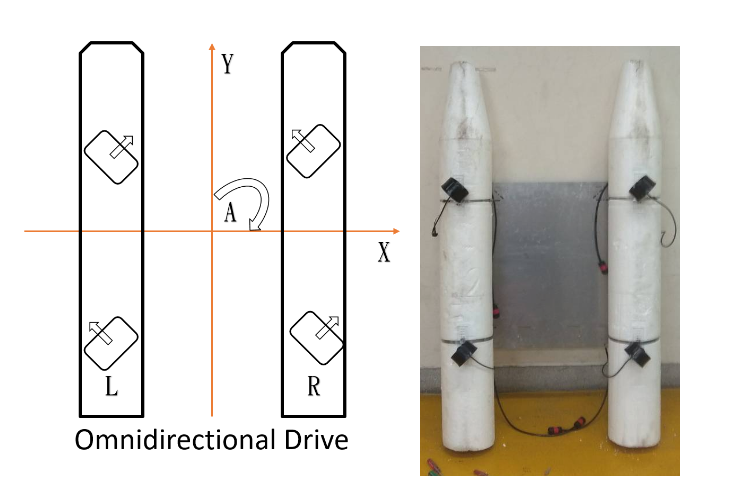
\includegraphics[width=1\columnwidth]{images/omni_drive.png}
	\centering
	\caption{omnidirectional drive motor config}
	\label{figure:omni_drive}
\end{figure}

\subsection{Conclusion}
We had already tried two different drive (Differential Drive and Omnidirectional Drive), the different drive can use in different environments, such as some areas have reefs and needs precise movement, we will prefer to use Omnidirectional Drive because we can avoid the boat hitting the rocks. Most of the time we will prefer to use Differential Drive because it consumes less power and more environmentally friendly.

